% !TeX spellcheck = es_VE
% !TeX root = Informe.tex
% !TeX spellcheck = es_VE
\documentclass[12pt,letterpaper]{article}
\usepackage[utf8]{inputenc}
\usepackage{amsmath}
\usepackage{amsfonts}
\usepackage{amssymb}
\usepackage{graphicx}
\usepackage{url}
\usepackage{tikz}
\usepackage[shortlabels]{enumitem} % Se mantiene aquí con sus opciones
\usepackage{fancyhdr}
\usepackage[spanish]{babel}
%\usepackage[acronym]{glossaries}
%\makeglossaries

% agregar circuitos electronicos
\usepackage[siunitx, american]{circuitikz}

% comas sencillas en listing
\usepackage{textcomp}
\usepackage{upquote}
\usepackage{listings}
\lstset{upquote=true}

% dimensiones de pagina
\usepackage[left=1.5cm,top=1.5cm,right=1.5cm,bottom=2.5cm]{geometry}

% hiperenlaces
\usepackage{hyperref} % Para incluir hipervínculos
\hypersetup{urlcolor=blue,colorlinks=false,pdfborder={0 0 0}} % eliminar marco rojo en enlaces (citas, indices, pies de pagina, etc)

% permitir en la numeracion de los items agregar el numero de seccion
% (Se eliminó la línea duplicada \usepackage{enumitem} que causaba el error)
\setlist[enumerate]{label=\thesection.\arabic*. }   % numerar solo con seccion
%\setlist[enumerate]{label=\thesubsection.\arabic*. } % incluir numeracion de subsection

% otras configuraciones
\usepackage{parskip}
\setlength{\parskip}{1em} % establece el espacio entre parrafos
\setlength{\parindent}{0cm} % elimina la sangria inicial en parrafo
\usepackage{array} % ajustes adicionales para tablas
% \usepackage{pdfpages} %incluir archivos pdf en documento

% personalizacion de etiquetas
\renewcommand{\figurename}{Figura}
\renewcommand{\contentsname}{Contenido}
\renewcommand{\listfigurename}{Índice de Figuras}
\renewcommand{\listtablename}{Índice de Tablas}
\renewcommand{\lstlistlistingname}{Índice de Códigos}
\renewcommand{\tablename}{Tabla}
\renewcommand{\lstlistingname}{Código}

% pie de pagina
\renewcommand{\footrulewidth}{0.4pt}% grosor de linea del pie de pag
%\lfoot{\thepage} % texto izquierda
%\rfoot{\thepage} % texto derecha
\cfoot{\thepage} % texto al centro

%% definiciones para insertar codigo de programacion al doc
\usepackage{color}
\definecolor{dkgreen}{rgb}{0,0.6,0}
\definecolor{gray}{rgb}{0.5,0.5,0.5}
\definecolor{mauve}{rgb}{0.58,0,0.82}
\lstset{frame=tb,
    language=Python,
    aboveskip=3mm,
    belowskip=3mm,
    showstringspaces=false,
    columns=flexible,
    basicstyle={\small\ttfamily},
    %numbers=left,
    numberstyle=\tiny\color{gray},
    keywordstyle=\color{blue},
    commentstyle=\color{dkgreen},
    stringstyle=\color{mauve},
    breaklines=true,
    breakatwhitespace=true,
    tabsize=3
} % fin de codigo de programacion

%%%%%%%%%%%%%% MACRO PARA CONTROL DE PUNTAJE %%%%%%%%%%%%%%%%%%
\usepackage{xifthen}
\newcounter{puntos}
\setcounter{puntos}{0} % Inicializa el contador a cero

\newcommand{\sumarPunto}[1]{%
    \addtocounter{puntos}{#1}%
    \ifthenelse{#1 > 1}{(\textbf{#1 puntos})}{(\textbf{#1 punto})} 
}
%%%%%%%%%%%%%%%%%%%%%%%%%%%%%%%%%%%%%%%%%%%%%%%%%%%%%%%%%%
\usepackage[T1]{fontenc}
\usetikzlibrary{arrows.meta,positioning,shapes.geometric,fit,calc,backgrounds}

%%%%%%%%%%%%%%%%%%%%%%%%%%%%%%%%%%%%%%%%%%%%%%%%%%%%%%%%%%%%%%%%%%%%%%%
\pagestyle{fancy}
\fancyhf{}

\setlength{\headheight}{80pt}
\addtolength{\topmargin}{-35pt}
\setlength{\headsep}{1cm}
\setlength{\footskip}{20pt}

\rhead{
\includegraphics[width=1.3cm]{../../img/logo_ciencias.png}}
\lhead{
\includegraphics[width=1.4cm]{../../img/logo_ucv.png}}
\cfoot{\thepage}
\rfoot{Noviembre, 2026}

\chead{Laboratorio de Internet de las Cosas}
\newcommand{\titulo}{PROYECTO FINAL}
\newcommand{\subtitulo}{Cuna inteligente con ESP32, MQTT y panel web}
\newcommand{\autorUno}{Luisdavid Colina V24766381}
\newcommand{\autorDos}{Samantha Ramírez V31307714}

% Las capturas van en la misma carpeta que el .tex para que \includegraphics las encuentre
\graphicspath{{./}{../vista_previa/}}
%%%%%%%%%%%%%%%%%%%%%%%%%%%%%%%%%%%%%%%%%%%%%%%%%%%%%%%%%%%%%%%%%%%%%%%
\begin{document}

\begin{center}
  {\Large \textbf{\titulo}} \\[0.3cm]
  {\large \textbf{\subtitulo}} \\[0.8cm]

  \small
  \begin{tabular}{c}
    \textbf{Preparado por:} \\
    \autorUno \\
    \autorDos \\
  \end{tabular}
  \\[1cm]
\end{center}

%%%%%%%%%%%%%%%%%%%%%%%%%%%%%%%%%%%%%%%%%%%%%%%%%%%%%%%%%%%%%%%%%%%%%%%
\section{Planteamiento}

Quien cuida a un bebé no puede estar siempre junto a la cuna. Durante la noche hay
tres situaciones que piden atención inmediata: el llanto, el pañal mojado y un cuarto
demasiado caliente o demasiado frío. Una cuna común no avisa de ninguna de las tres.

El proyecto propone una cuna que detecta esas situaciones, responde por sí sola con
un movimiento suave y avisa a los padres desde el teléfono. El trabajo se realizó
completo en simulación sobre Wokwi, con una placa ESP32 y un broker MQTT público.

Los objetivos son los siguientes.

\begin{enumerate}[label=\arabic*.]
  \item Detectar el llanto y mecer la cuna con una intensidad que crece si el llanto
        continúa.
  \item Medir la temperatura y la humedad del cuarto y controlar un ventilador.
  \item Avisar al teléfono cuando el pañal se moja, hay gas o humo, o el llanto se
        prolonga.
  \item Permitir mecer la cuna y manejar el ventilador a distancia desde un panel web.
\end{enumerate}

%%%%%%%%%%%%%%%%%%%%%%%%%%%%%%%%%%%%%%%%%%%%%%%%%%%%%%%%%%%%%%%%%%%%%%%
\section{Antecedentes}

Las cunas inteligentes son un tema frecuente en proyectos de IoT. Una lista de
proyectos para estudiantes de ingeniería incluye la cuna que mece al detectar el
llanto y vigila la temperatura del cuarto~\cite{robocraze}. Un proyecto publicado en
Intel DevMesh usa un ESP32 con un sensor de sonido, un DHT11 y un motor que inclina
la cuna, con alertas por la aplicación Blynk~\cite{devmesh}. Un proyecto de grado de
la Universidad Nacional An-Najah añade un sensor de humedad para el pañal, un
ventilador que se enciende cuando el cuarto supera los 30~°C y el control remoto del
mecido desde una aplicación~\cite{najah}.

Un artículo de 2025 describe un sistema más completo. Reporta niveles de balanceo del
1 al 5, parada automática del balanceo a los cinco minutos, un rango seguro de
temperatura de 20 a 25~°C con enfriamiento por encima y calefacción por
debajo, y un panel con historial y control remoto~\cite{pmc}. El mismo artículo
presenta cifras de exactitud que no son consistentes entre sus secciones, por lo que
este informe toma de él solo los parámetros de diseño y no sus resultados.

Un artículo de 2026 sobre una cuna con ESP32 y Blynk describe que el controlador
separa los ruidos breves del llanto verdadero para no mecer con cada sonido, y que la
cuna empieza a moverse en menos de 2,5 segundos tras confirmar el llanto~\cite{ijirt}.
De ahí sale la condición de duración mínima que usa este proyecto.

La cuna de este informe toma esos parámetros y añade cuatro elementos: un
escalonamiento de la respuesta según cuánto dura el llanto, un control con histéresis
para el ventilador, un panel que se maneja por MQTT con las mismas órdenes que
entiende el programa y un aviso al teléfono que no depende de tener el panel abierto.

%%%%%%%%%%%%%%%%%%%%%%%%%%%%%%%%%%%%%%%%%%%%%%%%%%%%%%%%%%%%%%%%%%%%%%%
\section{Diseño del sistema}

%%%%%%%%%%%%%%%%%%%%%%%%%%%%%%%%%%%%%%%%%%%%%%%%%%%%%%%%%%%%%%%%%%%%%%%
\subsection{Arquitectura}

El ESP32 lee los sensores y maneja los actuadores. Publica su estado en un broker MQTT
al instante cuando algo cambia, y además envía un latido cada segundo. El panel web se
suscribe a ese estado para mostrarlo. Las órdenes hacen el camino inverso: el panel
publica en un tópico de comandos y el ESP32 las recibe. Los avisos urgentes salen del
ESP32 por HTTP hacia ntfy, que los entrega al teléfono aunque el panel esté cerrado. La
figura~\ref{fig:arq} resume el flujo.

\begin{figure}[ht!]
\centering
\resizebox{\linewidth}{!}{%
\begin{tikzpicture}[
  node distance=7mm and 12mm,
  box/.style={draw, rounded corners=2pt, minimum height=8mm, align=center, font=\small, fill=white},
  grp/.style={draw, rounded corners=4pt, inner sep=6pt, fill=gray!8},
  arr/.style={-{Stealth[length=2mm]}, thick}
]
  \node[box] (dht) {DHT22};
  \node[box, below=of dht] (mpu) {MPU6050};
  \node[box, below=of mpu] (sl) {Sonido, peso,\\gas y pañal};
  \node[box, right=22mm of mpu, minimum height=50mm, minimum width=24mm, fill=blue!8] (esp) {ESP32};
  \node[box, below right=0mm and 22mm of esp.north east] (servo) {Servo};
  \node[box, below=of servo] (rele) {Relé y\\ventilador};
  \node[box, below=of rele] (otros) {Buzzer, LED\\y OLED};
  \node[box, right=26mm of rele, fill=orange!12] (broker) {Broker MQTT\\HiveMQ};
  \node[box, right=14mm of broker, fill=green!10] (panel) {Panel web\\en el teléfono};

  \draw[arr] (dht) -- (esp.west |- dht);
  \draw[arr] (mpu) -- (esp);
  \draw[arr] (sl) -- (esp.west |- sl);
  \draw[arr] (esp.east |- servo) -- (servo);
  \draw[arr] (esp.east |- rele) -- (rele);
  \draw[arr] (esp.east |- otros) -- (otros);
  \draw[arr] ([yshift=2mm]rele.east) -- node[above, font=\scriptsize]{estado} ([yshift=2mm]broker.west);
  \draw[arr] ([yshift=-2mm]broker.west) -- node[below, font=\scriptsize]{órdenes} ([yshift=-2mm]rele.east);
  \draw[{Stealth[length=2mm]}-{Stealth[length=2mm]}, thick] (broker) -- (panel);
  \node[box, below=30mm of broker, fill=orange!12] (ntfy) {ntfy};
  \node[box, right=14mm of ntfy, fill=green!10] (tel) {Teléfono};
  \draw[arr] (esp.south) |- node[below, font=\scriptsize, pos=0.75]{avisos por HTTP} (ntfy.west);
  \draw[arr] (ntfy) -- (tel);

  \begin{scope}[on background layer]
    \node[grp, fit=(dht)(mpu)(sl), label={[font=\scriptsize]above:Entradas}] {};
    \node[grp, fit=(servo)(rele)(otros), label={[font=\scriptsize]above:Salidas}] {};
  \end{scope}
\end{tikzpicture}}
\caption{Arquitectura del sistema. El estado sube al cambiar y con un latido por
segundo, las órdenes bajan por un tópico distinto y los avisos urgentes van al teléfono.}
\label{fig:arq}
\end{figure}

%%%%%%%%%%%%%%%%%%%%%%%%%%%%%%%%%%%%%%%%%%%%%%%%%%%%%%%%%%%%%%%%%%%%%%%
\subsection{Componentes y conexiones}

La tabla siguiente lista cada pieza del circuito, la magnitud que mide o la acción que
realiza, y el pin del ESP32 al que se conecta.

\begin{center}
\small
\begin{tabular}{llc}
\hline
\textbf{Pieza} & \textbf{Función} & \textbf{Pin} \\
\hline
DHT22                  & Temperatura y humedad del cuarto & 15 \\
MPU6050                & Movimiento de la cuna, por I2C   & 21 y 22 \\
Pantalla OLED SSD1306  & Estado de la cuna, por I2C       & 21 y 22 \\
Deslizante Sonido      & Nivel de ruido, de 0 a 4095      & 34 \\
Deslizante Peso        & Peso sobre el colchón, de 0 a 8 kg & 33 \\
Deslizante Gas         & Concentración de gas o humo      & 35 \\
Deslizante Pañal       & Humedad del pañal                & 32 \\
Servo                  & Mece la cuna                     & 18 \\
Módulo relé            & Enciende el ventilador           & 26 \\
LED rojo               & Alerta de llanto, pañal o gas    & 27 \\
Buzzer                 & Avisos sonoros                   & 25 \\
Cuatro botones         & Provocan situaciones de prueba   & 13, 14, 16 y 17 \\
\hline
\end{tabular}
\end{center}

El dibujo del circuito sigue dos reglas: cada pieza va del lado del ESP32 donde está su
pin, en el mismo orden, y la alimentación usa símbolos VCC y GND propios de cada pieza
en vez de llevar todos los cables a un solo pin. Así ningún cable cruza la placa, como
muestra la figura~\ref{fig:circuito}. Los símbolos VCC del simulador entregan 3,3~V:
cada deslizante recorre de 0 a 4095 en el convertidor sin saturarse.

\begin{figure}[ht!]
\centering
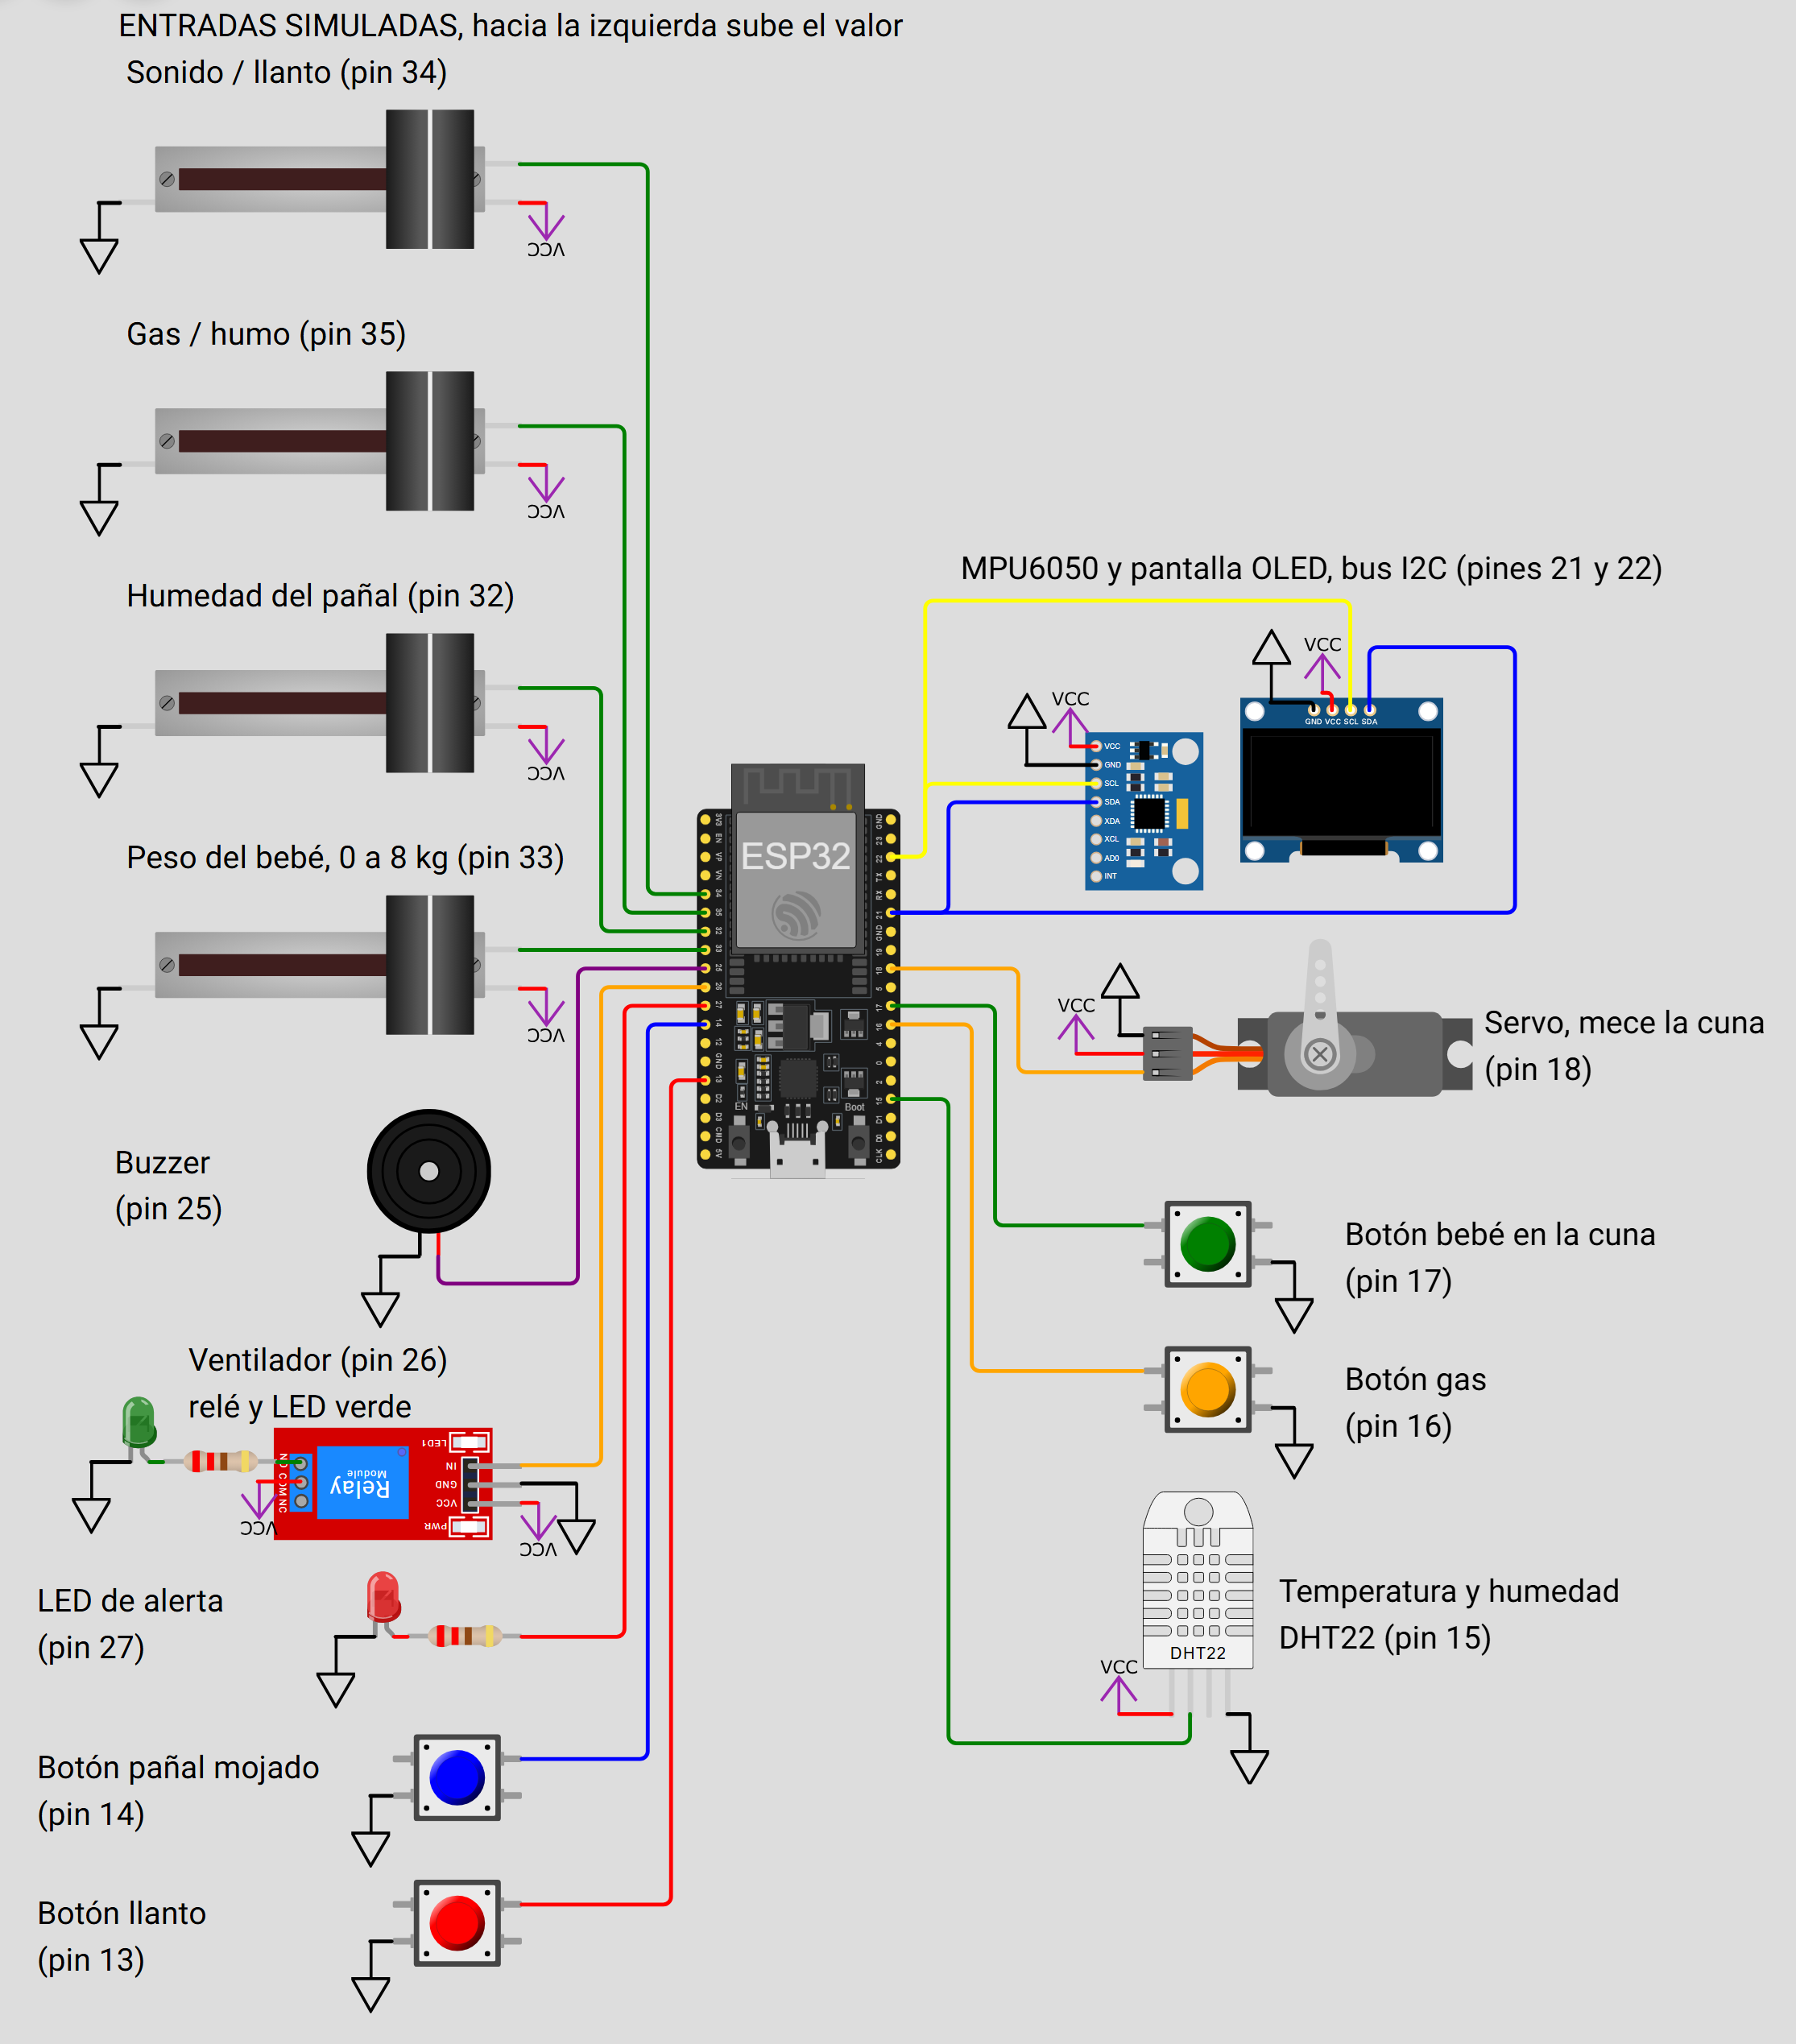
\includegraphics[width=0.62\linewidth]{circuito.png}
\caption{Circuito en Wokwi. Los deslizantes están girados para que su señal quede frente
al ESP32, por lo que su valor sube hacia la izquierda.}
\label{fig:circuito}
\end{figure}

%%%%%%%%%%%%%%%%%%%%%%%%%%%%%%%%%%%%%%%%%%%%%%%%%%%%%%%%%%%%%%%%%%%%%%%
\subsection{Sustituciones por las limitaciones del simulador}

La documentación de Wokwi no incluye un sensor de sonido entre sus piezas. Incluye el
amplificador de celdas de carga HX711, pero su valor solo se controla desde escenarios
de automatización y no con un control que se mueva a mano durante la
demostración~\cite{wokwihx}. El sensor de gas MQ2 sí existe, pero solo permite fijar
la concentración inicial~\cite{wokwigas}.

Por eso las cuatro entradas que representan sonido, peso, gas y humedad del pañal son
controles deslizantes que entregan un voltaje analógico. El programa las lee con el
convertidor del ESP32 y las trata como lo haría con los sensores reales. En un
montaje físico, el deslizante de sonido sería un micrófono con salida analógica, el de
peso una celda de carga con HX711, el de gas un MQ2 y el del pañal un sensor de
humedad. El resto de las piezas, como el DHT22, el MPU6050, el servo, el relé y la
pantalla OLED, sí existen en el simulador y se usan tal cual.

%%%%%%%%%%%%%%%%%%%%%%%%%%%%%%%%%%%%%%%%%%%%%%%%%%%%%%%%%%%%%%%%%%%%%%%
\section{Lógica de control}

%%%%%%%%%%%%%%%%%%%%%%%%%%%%%%%%%%%%%%%%%%%%%%%%%%%%%%%%%%%%%%%%%%%%%%%
\subsection{Respuesta al llanto}

El programa lee el sensor de sonido cada 200 ms, tomando el valor máximo de veinte
muestras para no perder los picos. Un ruido alto aislado no cuenta como llanto. Debe
mantenerse por encima del umbral durante dos segundos y, además, debe haber un bebé en
la cuna según la lectura de peso. Cumplidas las dos condiciones, la cuna empieza a
mecer con intensidad suave.

Si el llanto continúa, la respuesta escala. Al minuto el mecido pasa a intensidad
firme. A los tres minutos se avisa a los padres de un llanto prolongado, con una
alarma sonora, un mensaje al panel y una notificación al teléfono. Cuando el sonido baja
del umbral y se mantiene así durante veinte segundos, se da al bebé por calmado y el mecido se detiene. La
figura~\ref{fig:estados} muestra la secuencia.

\begin{figure}[ht!]
\centering
\begin{tikzpicture}[
  st/.style={draw, rounded corners=3pt, minimum width=27mm, minimum height=9mm, align=center, font=\small, fill=white},
  arr/.style={-{Stealth[length=2mm]}, thick},
  lb/.style={font=\scriptsize, align=center}
]
  \node[st, fill=green!10] (calm) {Tranquilo};
  \node[st, fill=orange!15, right=30mm of calm] (n1) {Llanto\\mecido suave};
  \node[st, fill=orange!25, right=30mm of n1] (n2) {Llanto\\mecido firme};
  \node[st, fill=red!15, right=30mm of n2] (alert) {Aviso a\\los padres};
  \node[st, fill=gray!15, below=22mm of n1] (rest) {Descanso\\del mecido};

  \draw[arr] (calm) -- node[below, lb]{ruido $\geq$ umbral\\por 2 s} (n1);
  \draw[arr] (n1) -- node[above, lb]{llanto\\por 60 s} (n2);
  \draw[arr] (n2) -- node[above, lb]{llanto\\por 180 s} (alert);
  \draw[arr] (n1.north) to[bend right=35] node[above, lb]{silencio por 20 s} (calm.north west);
  \draw[arr] (n1.south) -- node[right, lb]{mecido\\por 5 min} (rest.north);
  \draw[arr] (n2.south) to[bend left=20] node[right, lb, pos=0.35]{mecido\\por 5 min} (rest.east);
  \draw[arr] (n2.north) to[bend right=25] node[above, lb]{silencio por 20 s} (calm.north east);
  \draw[arr] (rest.west) to[bend left=60] node[left, lb, pos=0.5]{tras 2 min,\\si sigue\\el llanto} (n1.south west);
\end{tikzpicture}
\caption{Estados de la respuesta al llanto. El mecido se detiene siempre a los cinco
minutos y descansa dos minutos antes de poder reiniciarse solo. El aviso a los padres
no detiene el mecido.}
\label{fig:estados}
\end{figure}

El límite de cinco minutos aplica también cuando el balanceo se inicia a mano desde el
panel. Si el bebé sale de la cuna, el programa da el llanto por terminado y detiene el
mecido automático.

Esos tiempos no caben en una exposición, y menos en un simulador que corre más lento que
el tiempo real. Por eso existe un modo demo: se activa desde el panel, sin recompilar, y
divide todos los tiempos entre diez. Los valores de este informe son los del modo normal.

%%%%%%%%%%%%%%%%%%%%%%%%%%%%%%%%%%%%%%%%%%%%%%%%%%%%%%%%%%%%%%%%%%%%%%%
\subsection{Ambiente del cuarto}

El ventilador se enciende cuando la temperatura llega a 26~°C y se apaga al bajar a
24,5~°C. La diferencia de un grado y medio entre los dos valores evita que el relé se
active y se desactive sin parar cuando la temperatura oscila alrededor de un solo
umbral. El panel permite además forzar el ventilador encendido o apagado.

Se envía un aviso cuando la temperatura llega a 28~°C o baja a 20~°C, y otro cuando
la humedad cae por debajo de 40~\%. Cada aviso se emite una sola vez y se rearma
cuando la medida vuelve a un margen seguro, de modo que el panel no se llena de
mensajes repetidos.

El gas y el pañal también tienen rearme. La alarma de gas se activa con una lectura de
1800 y se apaga por debajo de 1400, y la del pañal se activa con 2000 y se apaga por
debajo de 1500. Al apagarse se publica un aviso de gas despejado o de pañal seco. El
MPU6050 vigila los golpes: una desviación de más de 0,5~g respecto a la gravedad genera
un aviso de movimiento brusco, que se rearma por debajo de 0,2~g.

\begin{center}
\small
\begin{tabular}{lll}
\hline
\textbf{Situación} & \textbf{Condición} & \textbf{Respuesta} \\
\hline
Llanto                 & Sonido alto por 2 s con bebé presente & Mecido suave \\
Llanto sostenido       & 60 s de llanto                        & Mecido firme \\
Llanto prolongado      & 180 s de llanto                       & Alarma y aviso \\
Calma                  & 20 s bajo el umbral                   & Detiene el mecido \\
Cuarto caliente        & 26~°C o más                           & Ventilador encendido \\
Cuarto fresco          & 24,5~°C o menos                       & Ventilador apagado \\
Temperatura fuera de rango & 28~°C o más, 20~°C o menos         & Aviso \\
Humedad baja           & Menos de 40~\%                        & Aviso \\
Pañal mojado           & Lectura sobre el umbral               & Aviso y pitido \\
Gas o humo             & Lectura sobre el umbral               & Aviso y alarma continua \\
Movimiento brusco      & Más de 0,5~g de desviación            & Aviso y LED \\
\hline
\end{tabular}
\end{center}

%%%%%%%%%%%%%%%%%%%%%%%%%%%%%%%%%%%%%%%%%%%%%%%%%%%%%%%%%%%%%%%%%%%%%%%
\section{Comunicación por MQTT}

El ESP32 se conecta a la red virtual \texttt{Wokwi-GUEST}, que no pide contraseña y
tiene salida a internet~\cite{wokwiwifi}. Desde ahí publica en el broker público de
HiveMQ mediante la librería PubSubClient. Todos los tópicos cuelgan de
\texttt{ucv6565/cuna/} seguido de un identificador propio, para que los mensajes de
este proyecto no se mezclen con los de otros que usen el mismo broker.

\begin{center}
\small
\begin{tabular}{lll}
\hline
\textbf{Tópico} & \textbf{Dirección} & \textbf{Contenido} \\
\hline
\texttt{.../state}   & Cuna al panel & Estado en JSON al cambiar y cada segundo, retenido \\
\texttt{.../event}   & Cuna al panel & Texto de cada aviso \\
\texttt{.../status}  & Cuna al panel & \texttt{online} u \texttt{offline}, retenido \\
\texttt{.../cmd}     & Panel a la cuna & Orden en texto, como \texttt{rock:2} \\
\hline
\end{tabular}
\end{center}

El estado se publica con la bandera de retención, de modo que un panel que se abre
después recibe de inmediato la última lectura. Ese dato puede ser viejo, así que el panel
lo muestra como último dato conocido y solo declara la cuna en línea cuando llega un
estado en vivo. El tópico \texttt{.../status} usa el último deseo de MQTT (LWT): al
conectarse la cuna publica \texttt{online} y le deja al broker el mensaje
\texttt{offline}, que el broker publica por ella si deja de responder.

Las órdenes que entiende la cuna son \texttt{rock:0} a \texttt{rock:3} para detener o
mecer, \texttt{fan:auto}, \texttt{fan:on} y \texttt{fan:off} para el ventilador,
\texttt{cry:} y \texttt{temp:} seguidos de un valor para cambiar los umbrales,
\texttt{beep} para probar el buzzer y \texttt{demo:on} o \texttt{demo:off} para el modo
demo. Las de simulación, como \texttt{sim:cry:1} y \texttt{sim:cry:0}, fijan un valor en
vez de alternarlo, y \texttt{sim:temp:27} fuerza una temperatura. Repetir cualquiera de
ellas no cambia nada, lo que permite al panel reintentarlas sin efectos secundarios.

La reconexión de WiFi y MQTT corre en una tarea aparte de FreeRTOS. Mientras dura, el
programa principal sigue leyendo los sensores, meciendo la cuna y haciendo sonar las
alarmas.

El broker público no tiene autenticación, así que cualquiera que conozca el
identificador podría leer el estado o enviar órdenes. Para una simulación académica es
aceptable. Un producto real necesitaría un broker propio con usuario, contraseña y
cifrado.

%%%%%%%%%%%%%%%%%%%%%%%%%%%%%%%%%%%%%%%%%%%%%%%%%%%%%%%%%%%%%%%%%%%%%%%
\section{Avisos al teléfono}

Los avisos de gas, llanto prolongado, pañal mojado y movimiento brusco salen del ESP32
por HTTP hacia el servicio ntfy~\cite{ntfy}, en el tema
\texttt{ucv6565-cuna-} seguido del identificador. Quien instala la aplicación y se
suscribe a ese tema los recibe aunque el panel esté cerrado. Se eligió sobre un bot de
Telegram porque no necesita token, que quedaría a la vista en el código público del
simulador. A cambio, cualquiera que conozca el nombre del tema puede leer los avisos.

El envío lo hace la misma tarea de red, a partir de una cola, para no detener el programa
principal. Cada tipo de aviso tiene un mínimo de 30~s entre envíos.

%%%%%%%%%%%%%%%%%%%%%%%%%%%%%%%%%%%%%%%%%%%%%%%%%%%%%%%%%%%%%%%%%%%%%%%
\section{Panel web}

El panel es una sola página HTML que se abre desde el teléfono o el computador. Se
conecta al mismo broker por WebSocket seguro y se suscribe a los tópicos de estado, de
avisos y de presencia. Separa el estado del broker del estado de la cuna, indica hace
cuánto llegó el último dato y estima a qué velocidad corre la simulación a partir del
tiempo de encendido del ESP32. Con la cuna fuera de línea atenúa los datos y desactiva
los controles.

Muestra el estado general de la cuna, una escena animada, las medidas de temperatura,
humedad, peso, sonido, gas, pañal y movimiento, el ángulo del servo, y el estado del LED
y del buzzer. Las alarmas de pañal y gas las decide el firmware: el panel las lee del
estado y no recalcula los umbrales, para no contradecir la histéresis.

Cada botón pasa por tres estados: pendiente, confirmado cuando el estado de la cuna
refleja la orden, y ``la cuna no respondió'' si tras tres intentos no hay confirmación.
Además de mecer y manejar el ventilador, permite cambiar los umbrales, probar el buzzer,
forzar la temperatura y activar el modo demo.

Hay una gráfica por cada medida, sobre el mismo eje de cinco minutos, con los huecos
visibles cuando faltan datos y una tabla con los mismos valores. Gráficas y avisos se
conservan al recargar. Un botón activa la notificación del navegador y un sonido para los
eventos críticos, solo mientras la página siga abierta.

La librería MQTT del panel va incluida en la carpeta del proyecto, de modo que la
página solo necesita conexión para llegar al broker.

%%%%%%%%%%%%%%%%%%%%%%%%%%%%%%%%%%%%%%%%%%%%%%%%%%%%%%%%%%%%%%%%%%%%%%%
\section{Resultados de la simulación}

Las pruebas se ejecutaron el 1 de noviembre de 2026 con el programa y el circuito
finales, en copias temporales del proyecto de Wokwi con un identificador propio. Un
script con Playwright manejó Wokwi y el panel publicado en Vercel desde un navegador sin
interfaz, y un cliente MQTT tomó los tiempos. Se agruparon en cinco escenarios. Cada
versión se midió en una sola corrida, por lo que los valores de tiempo cambian según el
equipo. Los escenarios con Wokwi CLI de la carpeta \texttt{pruebas/} no se repitieron con
esta versión porque requieren un token.

\subsection*{Escenario 1: tiempo real}

La tabla compara el programa anterior con el final. La causa de la lentitud no era el
broker, que respondió en una mediana de 234~ms ida y vuelta, sino la simulación: sin
ninguna pausa en \texttt{loop()} y con el estado saliendo cada 2~s del reloj simulado, un
dato podía tardar más de 20~s reales. Las mejoras fueron una pausa de 10~ms en cada ciclo,
publicar el estado al cambiar, dibujar la pantalla solo al cambiar, I2C a 400~kHz y
conectar el WiFi indicando el canal.

\begin{center}
\small
\begin{tabular}{lll}
\hline
\textbf{Medida} & \textbf{Antes} & \textbf{Después} \\
\hline
Velocidad en Wokwi, mediana             & 8~\%                      & 25~\% \\
Orden hasta el estado, mediana          & 4 de 5 sin llegar en 20~s & 1,10~s \\
Órdenes sin respuesta                   & --                        & 0 de 12 \\
Reconexiones al broker                  & 1 en unos 4 min           & 0 en 6 min \\
Panel con la simulación detenida        & En línea hasta 40~s       & Sin señal a los 16~s \\
Aviso de cuna apagada por LWT           & No existía                & 45~s \\
\hline
\end{tabular}
\end{center}

En la versión final, el tiempo de la orden al estado fue de 0,83~s como mínimo y 5,90~s
como máximo, con dos de las 12 órdenes por encima de 2~s. El primer dato tardó entre 70 y
87~s desde que se pulsa iniciar, sobre todo por la compilación. Al recargar el panel con
la simulación detenida, nunca indicó que la cuna estuviera en línea.

\subsection*{Escenario 2: respuesta al llanto con escalada}

Se corrió en modo demo, con los tiempos divididos entre diez, y con el bebé presente. El
mecido se había detenido a mano justo antes, para comprobar que esa pausa no bloquea la
demostración. La tabla muestra el momento de cada aviso desde que sube el sonido. El
tiempo simulado se lee del reloj del ESP32, con resolución de un segundo. La figura~\ref{fig:panel_c}
muestra el panel durante este escenario.

\begin{center}
\small
\begin{tabular}{llll}
\hline
\textbf{Aviso} & \textbf{Programado} & \textbf{Simulado} & \textbf{Reloj real} \\
\hline
Llanto detectado y mecido suave      & 0,2~s & menos de 1~s & 1,2~s \\
Mecido firme                         & 6~s   & 6~s          & 11,9~s \\
Llanto prolongado y aviso al teléfono & 18~s  & 18~s         & 32,2~s \\
Mecido detenido por el límite        & 30~s  & 30~s         & 53,2~s \\
Bebé calmado, 2~s tras bajar el sonido & --  & 33~s         & 57,6~s \\
\hline
\end{tabular}
\end{center}

Las duraciones sin dividir, de 60~s, 180~s y 5~minutos, no se ejecutaron de principio a
fin en el reloj normal. El filtro de ruidos sí se probó con los tiempos normales: tres
ruidos de hasta un segundo simulado no dispararon el llanto, y uno sostenido sí.

\begin{figure}[ht!]
\centering
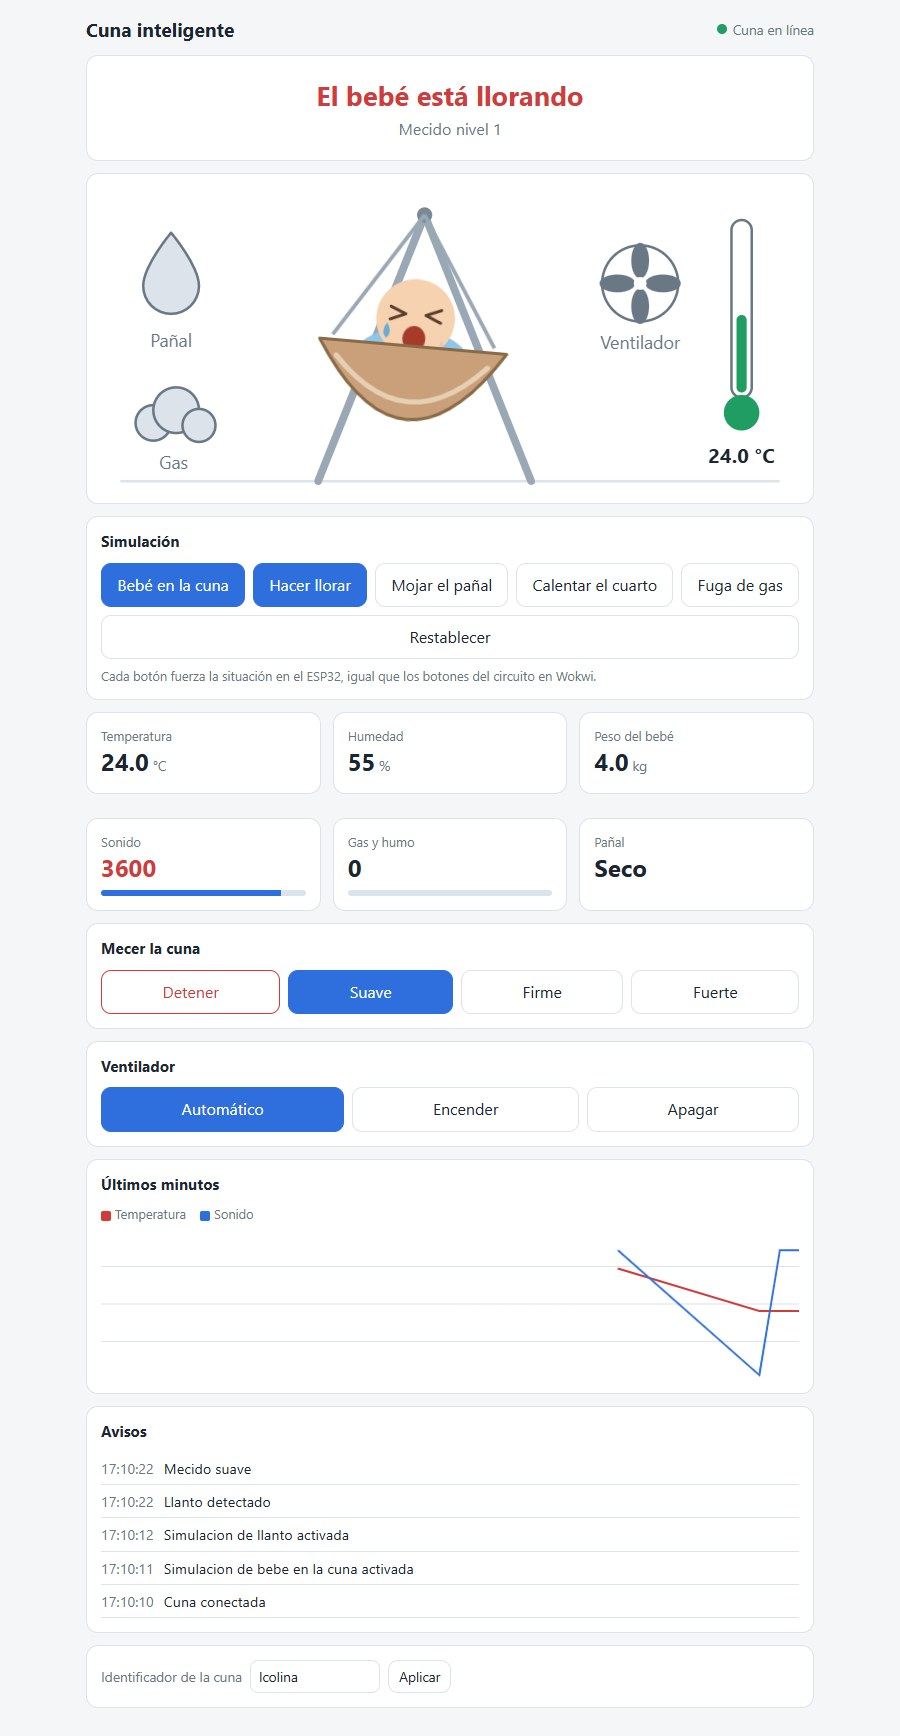
\includegraphics[width=0.5\linewidth]{panel_c_llanto.jpg}
\caption{Panel web en modo demo durante el llanto, con la cuna en línea y el mecido en
nivel 1.}
\label{fig:panel_c}
\end{figure}

\subsection*{Escenario 3: ventilador con histéresis}

Se forzó la temperatura a 24, 25, 27, 25 y 24~°C, en ese orden, y se leyó el estado del LED
verde en el simulador. A 25~°C, que está entre los dos umbrales, el ventilador siguió apagado
al subir y siguió encendido al bajar. Encendió a 27~°C y apagó a 24~°C. Moviendo el control del
DHT22 se repitió la bajada de 27 a 25 y 24~°C, con el mismo resultado. La
figura~\ref{fig:panel_d} muestra el panel con el ventilador activo y el aviso de pañal mojado.

\begin{figure}[ht!]
\centering
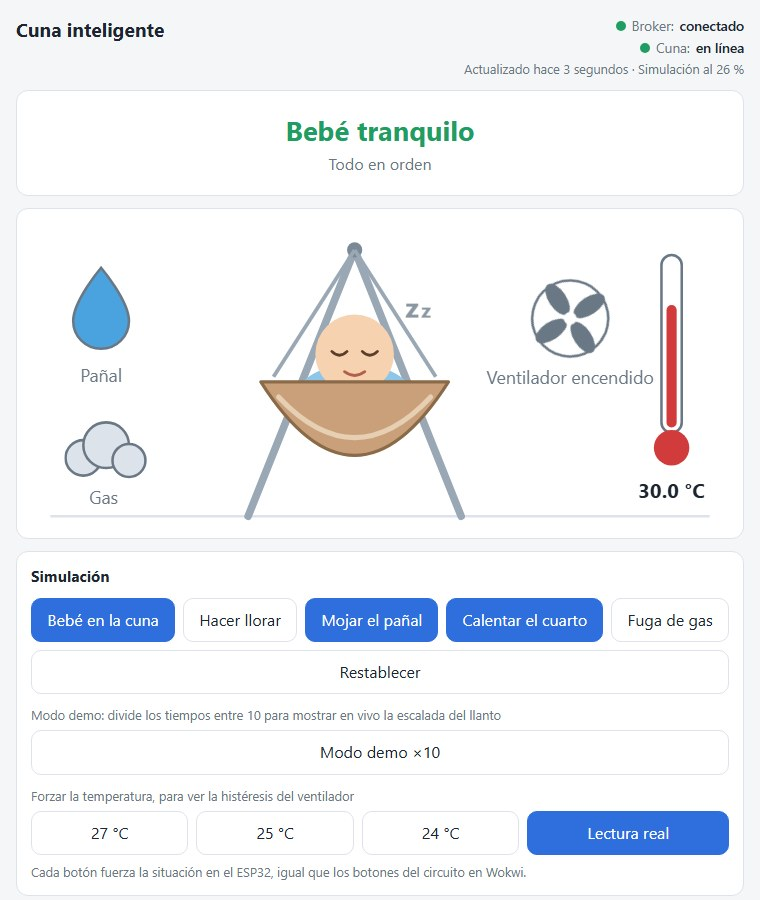
\includegraphics[width=0.5\linewidth]{panel_d_calor_panal.jpg}
\caption{Panel web con el ventilador encendido por calor forzado y el pañal mojado.}
\label{fig:panel_d}
\end{figure}

\subsection*{Escenario 4: gas, pañal y movimiento}

En cada paso se comparó la alarma del firmware, el LED rojo del simulador y lo que muestra
el panel, y coincidieron siempre. La lectura de gas se llevó a 2202, 1601 y 1201: la alarma
se activó, siguió activa entre el rearme y el umbral, y se apagó. La del pañal se llevó a
2402, 1801 y 1201, con el mismo comportamiento. Con 2~g en el MPU6050 se generó el aviso de
movimiento brusco con el LED rojo, y al volver a 1~g se rearmó. La figura~\ref{fig:panel_e}
muestra el panel durante la alerta de gas.

\begin{figure}[ht!]
\centering
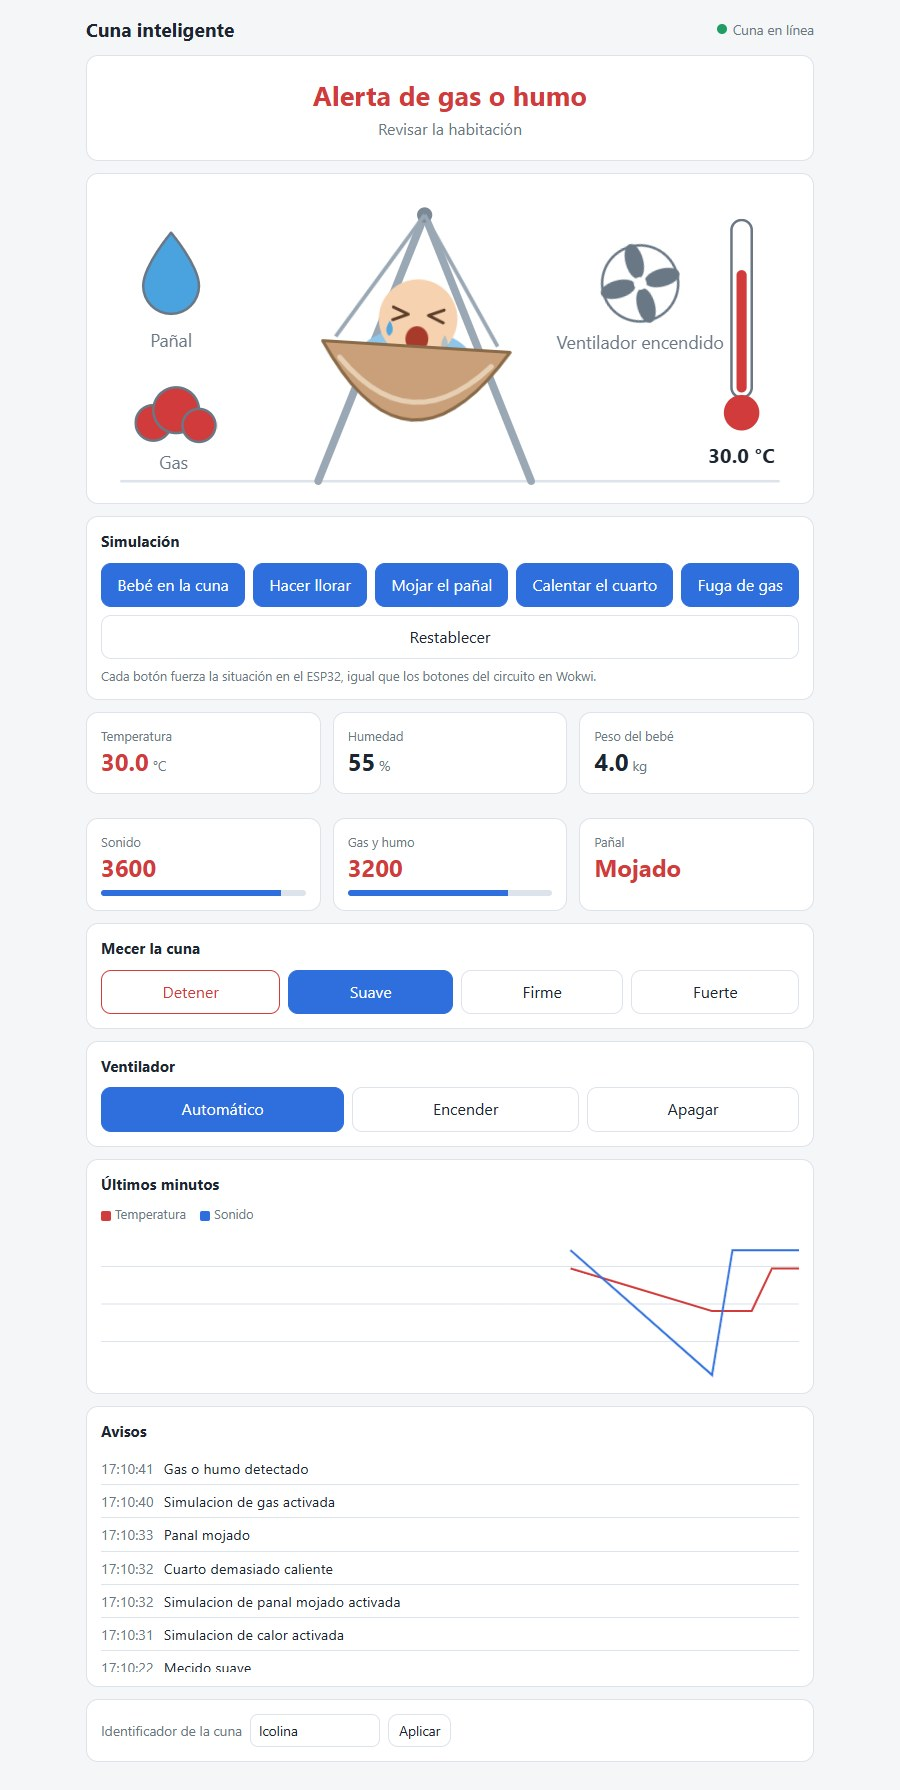
\includegraphics[width=0.5\linewidth]{panel_e_gas.jpg}
\caption{Panel web con la alerta de gas activa.}
\label{fig:panel_e}
\end{figure}

\subsection*{Escenario 5: avisos, controles y entradas}

Los cuatro tipos de aviso llegaron a ntfy, comprobados consultando el tema
(figura~\ref{fig:ntfy}). Durante un envío, con la alarma de gas sonando, el estado siguió
llegando con un máximo de 2,8~s entre mensajes y el servo siguió moviéndose. No se probó la
recepción en un teléfono físico.

Se probaron los cuatro botones del circuito y 28 usos de los controles del panel publicado,
y todos quedaron confirmados por el estado de la cuna. Los deslizantes de sonido, gas y
pañal leyeron 0, 2050 y 4095 al 0, 50 y 100~\% de su recorrido, y el de peso 0, 4 y 8~kg.

\begin{figure}[ht!]
\centering
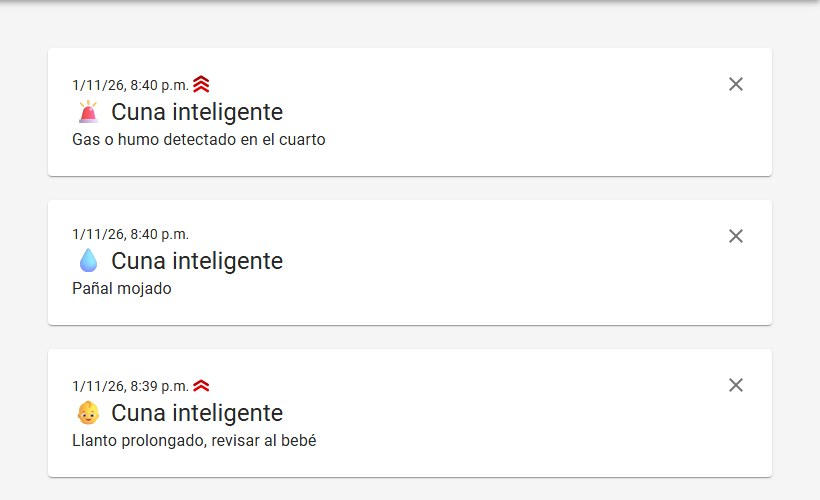
\includegraphics[width=0.6\linewidth]{ntfy_avisos.jpg}
\caption{Avisos recibidos en el tema de ntfy, vistos en su página web.}
\label{fig:ntfy}
\end{figure}

%%%%%%%%%%%%%%%%%%%%%%%%%%%%%%%%%%%%%%%%%%%%%%%%%%%%%%%%%%%%%%%%%%%%%%%
\section{Conclusiones}

\begin{enumerate}[label=\arabic*.]
  \item Una cuna que responde por escalones según la duración del llanto ignora los ruidos
        de menos de dos segundos y reserva el aviso al teléfono para los casos prolongados.
  \item El control con histéresis se comprobó en los dos sentidos: entre 24,5 y 26~°C el
        relé mantiene su estado anterior.
  \item El tiempo real en un simulador hay que medirlo. El broker no era el problema: con
        pausas en el programa y publicando al cambiar, la mediana de la orden al estado bajó
        de más de 20~s a 1,10~s.
  \item MQTT permite separar la cuna del panel. Los dos solo comparten el broker y el
        formato de los mensajes, y con el último deseo el panel distingue un dato en vivo de
        uno viejo.
  \item Las limitaciones del simulador se resolvieron con controles deslizantes
        equivalentes a las señales analógicas de los sensores reales, y esa
        sustitución queda declarada en el informe. Todo se verificó en simulación: los
        umbrales no están calibrados con sensores reales.
\end{enumerate}

%%%%%%%%%%%%%%%%%%%%%%%%%%%%%%%%%%%%%%%%%%%%%%%%%%%%%%%%%%%%%%%%%%%%%%%
\begin{thebibliography}{10}

\bibitem{robocraze} Robocraze, ``25 Creative IoT Lab Projects for Engineering
Students''. \url{https://robocraze.com/blogs/post/25-creative-iot-lab-projects-for-engineering-students}

\bibitem{devmesh} Intel DevMesh, ``Smart Cradle System''.
\url{https://devmesh.platformos.com/projects/smart-cradle-system}

\bibitem{najah} Universidad Nacional An-Najah, repositorio institucional, proyecto de
grado ``Comfort Sense baby bed'', 2024.
\url{https://repository.najah.edu/bitstreams/dd7b1d37-ed68-477b-893e-2b435eaeec99/download}

\bibitem{pmc} ``A novel smart baby cradle system utilizing IoT sensors and machine
learning for optimized parental care''. PubMed Central, 2025.
\url{https://pmc.ncbi.nlm.nih.gov/articles/PMC12125208/}

\bibitem{ijirt} P. S. Pise et al., ``IoT-Based Intelligent Baby Cradle'', International
Journal of Innovative Research in Technology, vol. 12, n.º 12, mayo de 2026.
\url{https://ijirt.org/publishedpaper/IJIRT202278_PAPER.pdf}

\bibitem{wokwiwifi} Wokwi Docs, ``ESP32 WiFi Networking''.
\url{https://docs.wokwi.com/guides/esp32-wifi}

\bibitem{wokwihx} Wokwi Docs, ``wokwi-hx711''.
\url{https://docs.wokwi.com/parts/wokwi-hx711}

\bibitem{wokwigas} Wokwi Docs, ``wokwi-gas-sensor''.
\url{https://docs.wokwi.com/parts/wokwi-gas-sensor}

\bibitem{ntfy} ntfy, ``Send push notifications to your phone or desktop via PUT/POST''.
\url{https://docs.ntfy.sh/}

\end{thebibliography}

\end{document}
